\documentclass[tikz, border=10pt]{standalone}
\usepackage[T1]{fontenc}
\usepackage[utf8]{inputenc}
\usepackage{lmodern}
\usepackage[table]{xcolor}
\definecolor{IntelBlue}{HTML}{0068B5}
\definecolor{IntelLightBlue}{HTML}{DDEEF9}
\definecolor{FpgaOrange}{HTML}{E67E22}
\definecolor{FpgaLight}{HTML}{FDEBD0}
\definecolor{HpsGreen}{HTML}{1A7A4A}
\definecolor{HpsLight}{HTML}{D5F5E3}
\definecolor{GrayBg}{HTML}{F2F3F4}
\definecolor{GrayBorder}{HTML}{AAB7B8}
\definecolor{PassGreen}{HTML}{D5F5E3}
\definecolor{PassGreenDark}{HTML}{1E8449}
\definecolor{RowAlt}{HTML}{F7F9FB}
\definecolor{SummaryBg}{HTML}{EBF5FB}
\definecolor{NodeFill}{HTML}{D6EAF8}
\definecolor{NodeBorder}{HTML}{1B4F72}
\definecolor{InitFill}{HTML}{E5E7E9}
\definecolor{InitBorder}{HTML}{717D7E}
\definecolor{SleepFill}{HTML}{FEF5E7}
\definecolor{SleepBorder}{HTML}{935116}
\definecolor{MsgFill}{HTML}{D1F2EB}
\definecolor{MsgBorder}{HTML}{0E6655}
\definecolor{TimeoutRed}{HTML}{C0392B}
\definecolor{BtnBlue}{HTML}{1A5276}
\definecolor{ArrowGray}{HTML}{717D7E}
\usepackage{tikz}
\usetikzlibrary{shapes.geometric, arrows.meta, positioning, fit, backgrounds, calc, decorations.pathreplacing, bending, shadows.blur}
\begin{document}
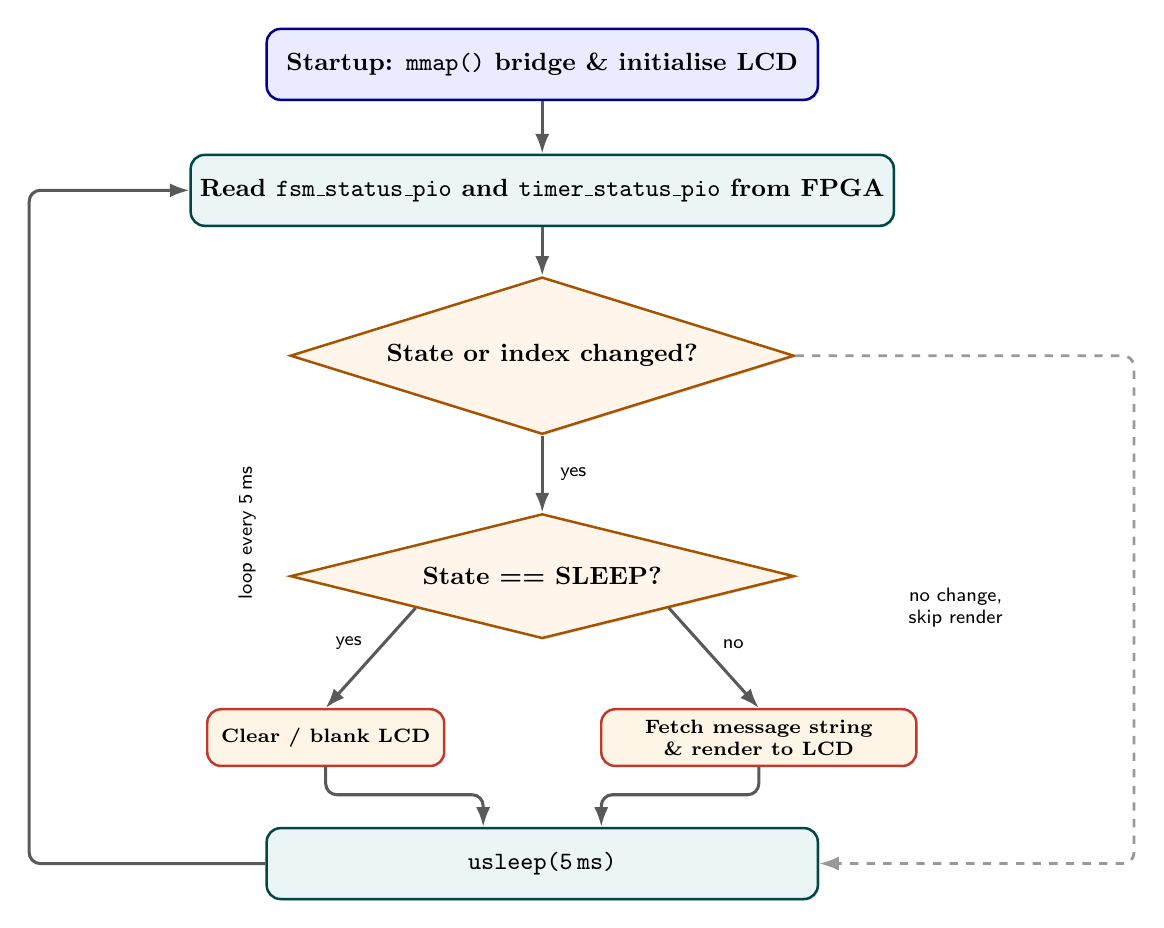
\begin{tikzpicture}[
  every node/.style={font=\small\sffamily},
  once/.style={
    rectangle, rounded corners=5pt,
    draw=blue!55!black, line width=0.9pt, fill=blue!8,
    minimum width=7cm, minimum height=0.9cm,
    align=center, font=\small\bfseries,
    drop shadow={shadow xshift=0.6pt, shadow yshift=-0.6pt, opacity=0.25}},
  loop/.style={
    rectangle, rounded corners=5pt,
    draw=teal!55!black, line width=0.9pt, fill=teal!8,
    minimum width=7cm, minimum height=0.9cm,
    align=center, font=\small\bfseries,
    drop shadow={shadow xshift=0.6pt, shadow yshift=-0.6pt, opacity=0.25}},
  cond/.style={
    diamond, aspect=2.6,
    draw=orange!65!black, line width=0.9pt, fill=orange!8,
    minimum width=6.4cm, minimum height=0.9cm,
    align=center, font=\small\bfseries, inner sep=2pt,
    drop shadow={shadow xshift=0.6pt, shadow yshift=-0.6pt, opacity=0.25}},
  upd/.style={
    rectangle, rounded corners=5pt,
    draw=TimeoutRed, line width=0.9pt, fill=SleepFill,
    minimum height=0.72cm,
    align=center, font=\scriptsize\bfseries,
    inner xsep=5pt, inner ysep=2pt,
    drop shadow={shadow xshift=0.45pt, shadow yshift=-0.45pt, opacity=0.18}},
  blankupd/.style={upd, minimum width=2.9cm},
  renderupd/.style={upd, text width=3.65cm},
  arr/.style={
    -{Latex[length=2.5mm,width=1.8mm]},
    draw=black!65, line width=1.1pt, rounded corners=4pt},
  darr/.style={
    -{Latex[length=2.5mm,width=1.8mm]},
    draw=black!40, line width=1.0pt, dashed, rounded corners=4pt},
  lbl/.style={font=\scriptsize\sffamily, fill=white, inner sep=2pt, rounded corners=2pt},
]

\node[once] (init) at (0,  0.0)
  {Startup: \texttt{mmap()} bridge \& initialise LCD};

\node[loop] (poll) at (0, -1.6)
  {Read \texttt{fsm\_status\_pio} and \texttt{timer\_status\_pio} from FPGA};

\node[cond] (chk)  at (0, -3.7)
  {State or index changed?};

\node[cond] (slpchk) at (0, -6.5)
  {State == SLEEP?};

\node[blankupd] (blank) at (-2.75, -8.55)
  {Clear / blank LCD};

\node[renderupd] (upd) at (2.75, -8.55)
  {Fetch message string \& render to LCD};

\node[loop] (slp)  at (0, -10.15)
  {\texttt{usleep(5\,ms)}};

\draw[arr] (init.south) -- (poll.north);
\draw[arr] (poll.south) -- (chk.north);

\draw[arr] (chk.south) -- node[lbl,right=4pt]{yes} (slpchk.north);
\draw[arr] (slpchk.south west) -- node[lbl,above left=1pt]{yes} (blank.north);
\draw[arr] (slpchk.south east) -- node[lbl,above right=1pt]{no} (upd.north);
\draw[arr] (blank.south) -- ++(0,-0.35) -| ([xshift=-0.75cm]slp.north);
\draw[arr] (upd.south)  -- ++(0,-0.35) -| ([xshift=0.75cm]slp.north);

\draw[darr]
  (chk.east)
  -- ++(4.3, 0)
  -- ++(0, -6.45)
  -- (slp.east);
\node[lbl, align=center] at (5.25, -6.9)
  {no change,\\skip render};

\draw[arr]
  (slp.west)
  -- ++(-3.0, 0)
  -- ++(0,  8.55)
  -- (poll.west);
\node[lbl, rotate=90, align=center] at (-3.75, -5.95) {loop every 5\,ms};

\end{tikzpicture}
\end{document}
